\section{METODOLOGIA DE PESQUISA}

Neste capitulo foi feita uma abordagem sobre como atender as
necessidades do usuário, identificando, analisando e deliberando a cerca da
causa raiz do problema. Foram examinadas as diversas etapas da
elaboração do sistema, para de fato atender o objetivo do projeto com
a finalidade de assegurar uma comunicação segura e eficiente.

Para tal objetivo, o desenvolvimento do sistema foi encaminhado em fases
que envolvem tanto aspectos visuais quanto estruturais. Buscou-se,
inicialmente, idealizar uma interface gráfica que facilitasse a
interação do usuário, ao mesmo tempo em que se projetava a estrutura
técnica responsável pela comunicação segura, sendo esta a proposta
central do projeto.

\subsection{Arquitetura de Comunicação}

Apresentando nosso servidor e aplicação que oferecem uma solução robusta
e eficiente para a comunicação segura entre clientes, mostraremos
como as aplicações de mercado deveriam se comportar no nível superior
aos cuidados de segurança da informação. A estrutura da nossa
aplicação é composta por duas etapas fundamentais que garantem um
processo de conexão transparente e seguro. Inicialmente, os clientes
solicitam o endereço \acs{IP} externo de forma transparente, enquanto o
servidor cuida da gestão dessa informação por meio de uma chave
aleatória gerada e armazenada no \textit{\gls{back-end}}.

A função da chave é armazenar o identificador do destino de forma
segura, uma vez onde eu não mostro o endereço \acs{IP} do cliente
diretamente ao usuário, eu deixo sua confidencialidade preservada.

\begin{figure}[H]
  \centering
  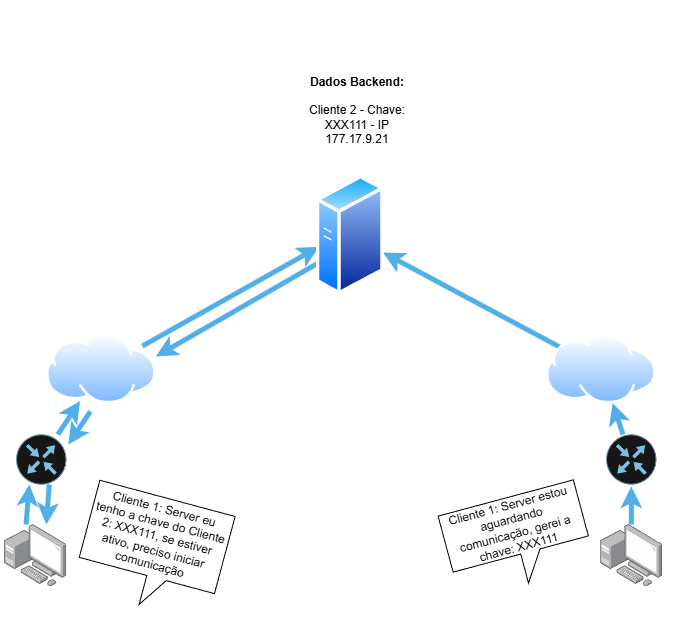
\includegraphics[width=0.8\linewidth]{imagens/arquitetura-etapa1.png}
  \caption[Primeira etapa da conexão com o servidor, onde o
    cliente solicita ao servidor que o conecte com o usuário de
  destino]{O cliente solicita ao servidor que o conecte com o usuário
  de destino.}
  \label{fig:arquitetura_etapa1}
\end{figure}

O cliente tendo a chave em mãos, tentará estabelecer uma conexão
com o destino. Se este estiver online, o servidor atua como um
identificador exclusivo, assegurando que a comunicação seja iniciada
de maneira controlada e segura.

À medida que as mensagens são trocadas, elas transitam exclusivamente
pelo servidor, que se torna o meio principal para a interface com o
destinatário. Importante destacar que toda comunicação realizada
através do nosso sistema é criptografada. Isso significa que os dados
não são armazenados pelo servidor durante sua transferência, em vez
disso, ele simplesmente transporta a informação até a outra ponta de
forma ágil e segura.

\begin{figure}[H]
  \centering
  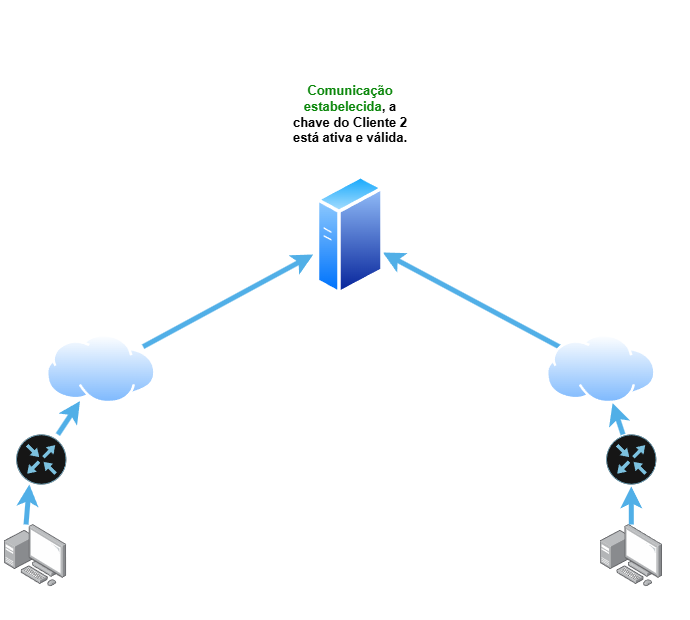
\includegraphics[width=0.8\linewidth]{imagens/arquitetura-etapa2.png}
  \caption[Segunda etapa da conexão com o servidor, a comunicação é
  estabelecida com sucesso entre ambos os usuários]{A comunicação é
  estabelecida com sucesso entre ambos os usuários.}
  \label{fig:arquitetura_etapa2}
\end{figure}

No encerramento da comunicação na 3ª etapa, a aplicação informa ao
servidor para iniciar a contagem de 12 horas para exclusão da chave e
do \acs{IP} externo do usuário, caso não haja interação durante esse
período pós fechamento da aplicação.

\begin{figure}[H]
  \centering
  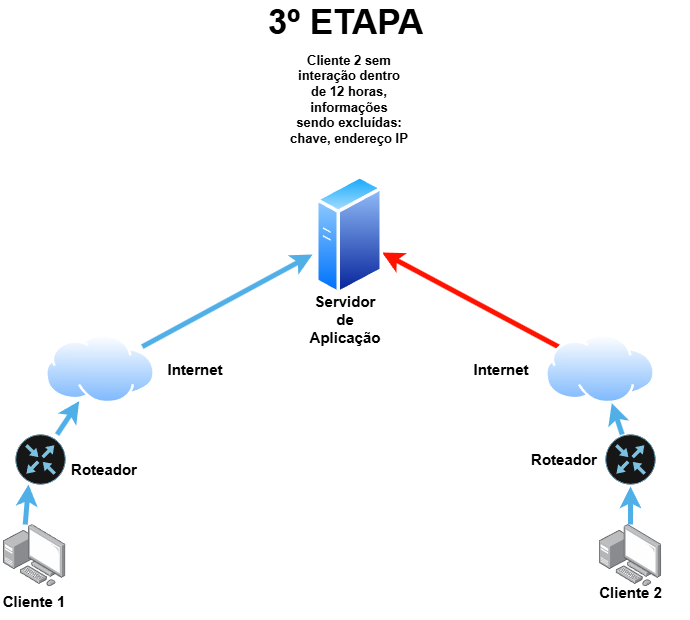
\includegraphics[width=0.8\linewidth]{imagens/arquitetura-etapa3.png}
  \caption[Terceira etapa da conexão com o servidor, os usuários são
  desconectados após 12 horas de inatividade]{Os usuários são
  desconectados após 12 horas de inatividade.}
  \label{fig:arquitetura_etapa3}
\end{figure}

\subsection{Prototipagem da Interface Gráfica}

Como parte do processo metodológico, esta fase foi construída com o
intuito de antecipar a interação entre o usuário e o sistema. Esta
etapa permitiu visualizar e validar, de maneira preliminar, a
estruturação dos elementos visuais, fluxos de navegação e
funcionalidades básicas, antes da formação definitiva da aplicação.

A prototipagem contribui diretamente para a identificação de
melhorias na experiência do usuário, da comunicação entre os
integrantes da equipe e como ferramenta de análise das necessidades
práticas do projeto. A partir dessa ambientação visual, foi possível
ajustar funcionalidades e alinhar as decisões de design às metas de
confiabilidade e usabilidade do sistema. Este levantamento está
parelelo com os princípios da metodologia ágil, ao unir interações
rápidas e feedback contínuo, promovendo um processo de
desenvolvimento centrado no usuário e tecnicamente fundamentado.

\newpage
